\documentclass[a4paper,12pt]{article}
\usepackage[T1]{fontenc}
\usepackage{imakeidx}
\usepackage{graphicx}
%\makeindex[columns=3, title=Alphabetical Index, intoc]

\begin{document}

\textbf{Daniele Della Cioppa}

\textbf{Software Developer}

\tableofcontents
\clearpage

\section{Knowledge unit}

This is what I've been covering so far during the apprenticeship:

\begin{itemize}
\item {database development}
\item {application life cycle}
\item docker
\item github 
\item LateX
\item PostgreSQL
\item Linux
\item {iOS \& Android development}
\end{itemize}
\clearpage

\subsection{iOS \& Android development}
This is the stage I was at, on the 23rd March, with the mobile development since this is being literally self taught

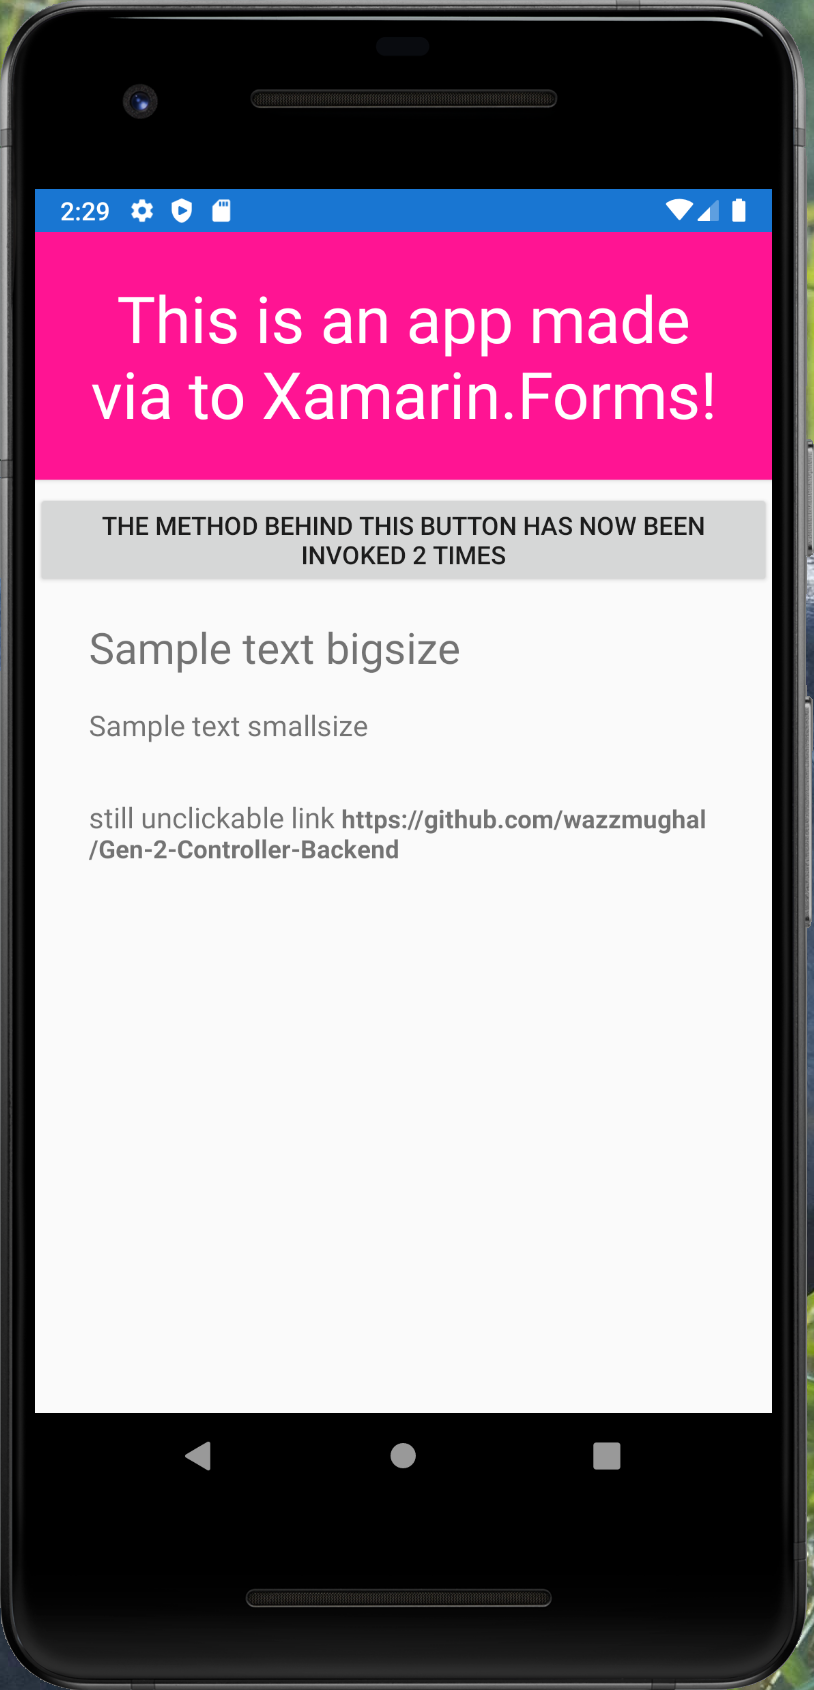
\includegraphics[width=9cm]{./capture-app.PNG}

We realized Xamarin brings in some difficulties even experts are struggling with. Since I'm on an apprenticeship we agreed to make it simple and use Android Studio to make an app for Android and later on use XCode for Apple. The problem with Apple is we'll need a real physical iPhone to test the app on

 

\section{Introduction}

After three months in my role I'm now responsible for the following tasks with databases:

\begin{itemize}
\item {reading the specs}
\item design
\item implementation
\item testing 
\item documenting
\end{itemize}

\clearpage

\subsection{design}
This is a first idea of the database I came up with

\noindent \includegraphics[width=14cm]{./ERSchemaGen2.jpg}

We agreed it was holding probably more information than what we need to display in the app so I came up later on with a smaller design which really has just the right amount of things we need to make sure we can run enough tests and see how the App, the Server and the Database interact between each other
\clearpage

This is the smaller database designed again from scratch. We need to add geolocation to nodes but for the time being it will be hard coded in the server and we'll try to see if we can display a hardcoded geolocation hold by the server to be caught by the client and displayed properly on the app

\noindent 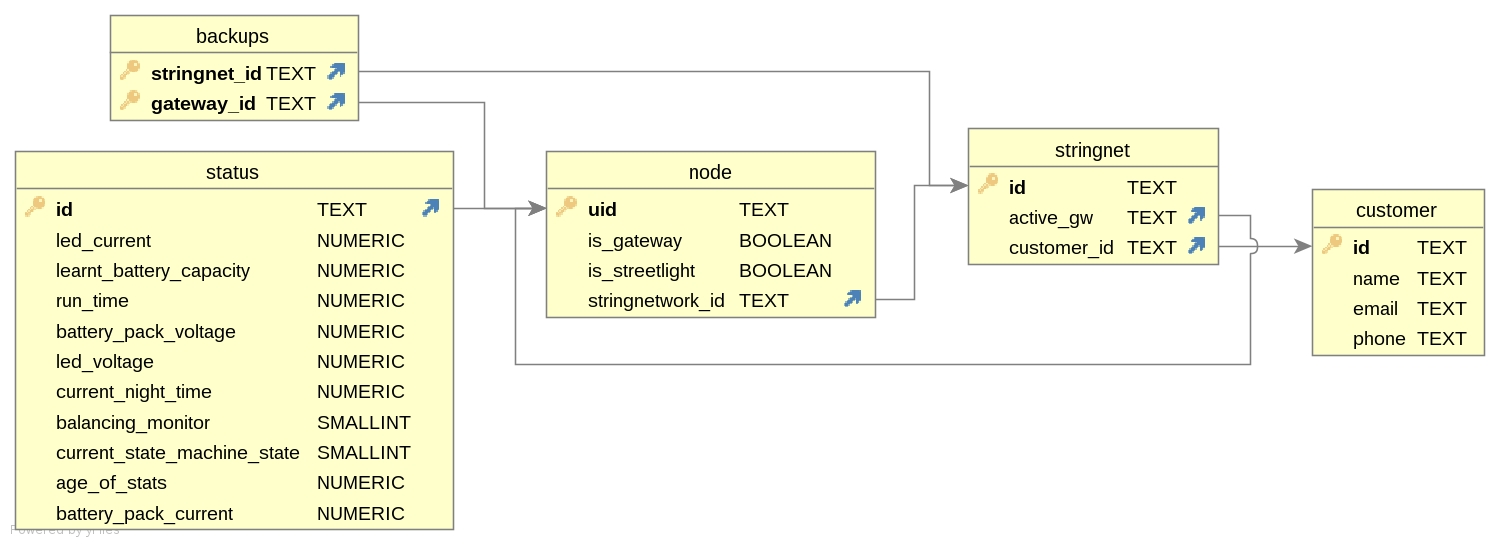
\includegraphics[width=14cm]{./SecondERSchemaGen2.jpg}

\printindex

\end{document}
